\ofsection{Gameplay}
%
\ofquote{"You want quiet, you better take the next train."\\}{Lightning}
%
\begin{center} 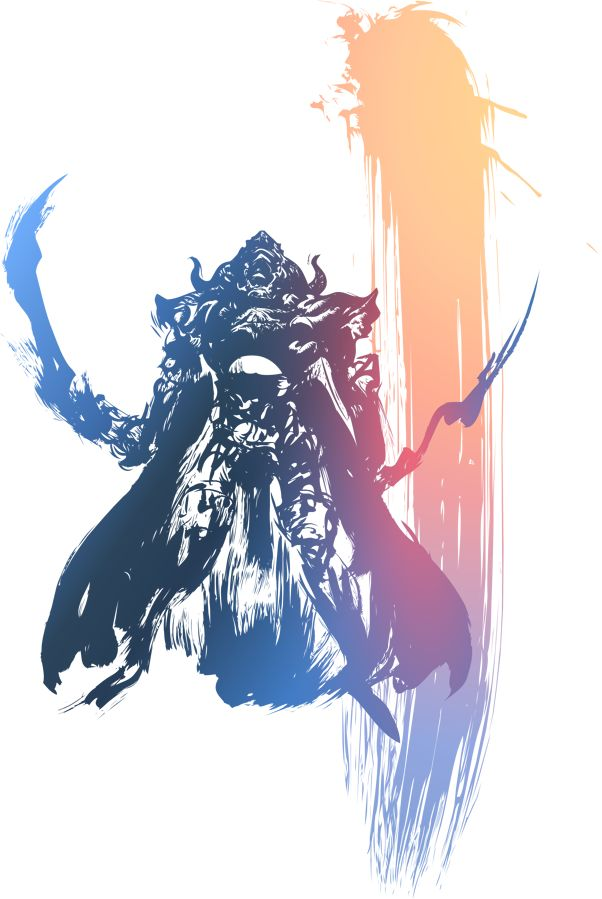
\includegraphics[width=\columnwidth]{./art/images/ff12.jpg} \end{center}
%
\accf{Final Fantasy} is a series of video games where each title features its unique story, world and characters.
Still they are part of the same series, not only due to recurring elements, but also because the stories focus on a group of heroes who face a great conflict.
\accf{Omega Fantasy} is a tabletop game that helps you to create Final Fantasy adventures with your friends and this release, named Omega~Fantasy~II, is an improved version of the original release.
To play, you only need dice, paper, pens, this book and at least one friend, but a group size of 4 to 6 is recommended.
To complete an adventure, your group needs to meet one or more times and play the game, each such gathering is called a \accf{Session}.
%
\ofpar
%
Choose one person to become the \accf{Game Master}~(shortened~\accf{GM}), who creates the game world and narrates the adventure by using the content and guidelines in this book.
During the game, he describes the environment to the players and how it reacts to their actions. 
The GM also takes the role of all non-player characters to narrate conversations and combat. 
Everyone else is a \accf{Player}, who creates and plays the game from the perspective of a \accf{Character} in the game world.
Player characters are the protagonists of the story who travel together as a \accf{Party} to explore the world, interact with people and fight against enemies. 
%Usually, the party is confronted with a central conflict by the GM, as the general goal of their adventure.
%You do not need any prior knowledge of Final Fantasy or roleplaying, everything necessary is explained in the following.
This book divided into three major sections: this first section explains the core rules and gameplay elements.
The second section details rules for creating and developing characters.
The final section focuses on the GM and offers a wide variety of guidelines and content for creating a game world. 
%
\vfill
%
\ofboxwithtitle{Example: Roleplaying\vspace*{0.15cm}}
{
	\newcommand{\nl}{\vspace{0.2cm}\\}
	\acc{Hironobu (Game Master):} You enter the Thunder Plains, which is a vast wasteland covered by thick fog and dark clouds.
	The locals have erected towers, that act as lightning rods, but you can see that lighting bolts often strike the ground in the open field.\nl
	\acc{Yoshinori (playing as Wakka):} We head north, not too near and not too far from the towers, ya?\nl
	\acc{Nobuo (playing as Rikku):} I wanna go home! I hate lightning! I hate thunder!\nl
	\acc{Tetsuya (playing as Auron):} This storm never stops. Better to cross quickly.\nl
	\acc{Hironobu (Game Master):} You can also see a small building nearby, that looks like an inn.\nl
	\acc{Nobuo (playing as Rikku):} Let’s go rest over there! Please? I'm too young to die!\nl
	\acc{Tetsuya (playing as Auron):} Fine, we rest. She is worse than the storm.
}
%
\vfill
%
Dice rolls are used in various situations to help decide the outcome of uncertain actions, but their exact nature depends on the context. 
This game uses only six-sided dice and we use \accf{d} shorthand to refer to such a die.
Furthermore, we use for example 4d to describe a roll of 4 dice, where the result is the sum of all rolled dice.
\accf{Checks} are the main tool to help the GM to decide and narrate the outcome of actions.
He can either ask players for checks or perform them himself in secret.
Checks are usually \accf{2d} rolls and higher numbers mean a better outcome for the roller. 
The minimum result required to succeed is called Difficulty~(shortened \accf{DC}) and often has to be decided by the GM.
He should base this DC on the difficulty of the action itself and the proficiency of the actor in it.
Most DCs vary between 5 and 9, ones below that range are considered easy, while ones above it are very challenging.
%
\ofpar
%
Since checks are 2d rolls, the lowest and highest possible results are 2 and 12 respectively, which can be treated as unexpectedly good or bad, but still plausible outcomes.
A check can also have \accf{Advantage} or \accf{Disadvantage} when the circumstances have a substantial effect on the attempted action. 
In both cases, the check is made with 3d and with Advantage only the two highest and with Disadvantage only the two lowest dice are counted. 
Advantage and Disadvantage cancel each other out and do not stack.
%
%\ofpar
\clearpage
%
\ofboxwithtitle{Example: Advantage \& Disadvantage}
{
	Cloud meets Don Corneo in his mansion wearing a dress and make-up to convince him that he is a woman.
	The GM decides that this is a very difficult task (DC 10), because Cloud did not put much effort into his disguise. 
	But as the room is not well lit and the Don had a bit too much to drink, he also decides that the check has Advantage. 
	Cloud rolls 3d with the result [6,2,6] and since only the two highest dice count, he rolled the best possible outcome! 
	The GM decides that Don Corneo is not only convinced that Cloud is a woman, but he finds him so irresistible that he drags Cloud into his room for some time alone.
}
%
\ofpar
%
Another way to modify checks is through the use of \accf{Fortune Dice}.
At the start of each session, every player and the GM roll 1d and all results are written down and become the pool of Fortune Dice for this session.
During the session, after a player makes a roll, he or she can decide to remove one Fortune Die from the pool and use it to replace one die in the result of the roll.
However, the GM is also allowed to use Fortune Dice to modify the result of player rolls in the same manner.
This allows players to benefit from occasional strokes of luck or motivation while the GM can create moments of misfortune or complications.
In both cases, the person using the Fortune Die should try to give a narrative description of its effect.
Fortune Dice that are not used, are discarded at the end of each session.
%
\ofpar
%
\ofboxwithtitle{Example: Fortune Dice}
{
	Luneth explores the ancient Altar Cave. 
	As he walks towards a hole in the ground, the GM asks him for a DC~5 check to decide whether he can notice and avoid it.
	Luneth rolls [3, 4], which would pass the check.
	However, the GM decides to use a Fortune Die on his roll, the current pool of Fortune Dice includes \mbox{[1, 3, 3, 5]}.
	He removes the 1 from the pool and puts it in place of the 4 in Luneth's roll.  
	Accordingly, the roll is changed to [3, 1], which fails the check, and the remaining dice pool contains \mbox{[3, 3, 5]}.
	The GM describes this effect as follows: as he tries to carefully step around the hole, Luneth steps on a slippery rock, trips and falls into the hole.
	As a consequence, he finds himself an unknown and dangerous section of the cave and has find his way back to the exit.
}
%
\ofpar
%
\ofquote{"Why not? Nothing to lose but my life and I got that for free!"}{Setzer}\\\\
%
The party can explore the environment described by the GM at will.
They can look for specific things or wander around, but an appropriate amount of time passes while doing so.
The GM may draw a map of the party's current location as a visual aid. 
He is also free to impose checks on all exploration related actions, such as picking locks or detecting traps.
The party may go to sleep once per day to fully recover their HP and MP, even if unconscious.
To gain this benefit, they have to sleep in a comfortable place like an Inn or a Tent for multiple hours.
Throughout the adventure, the party will interact with other characters.
These non-player characters are voiced by the GM and accordingly the players talk from the perspective of their own characters.
To avoid confusion, it is important to clarify whether something you say is from the perspective of your character or from yours as player or GM.
During conversations, the GM may ask for checks, for example to decide whether an attempt to convince a character is successful.
%
\vfill
%
\ofquote{"You know what they say about the leading man, don't you? He never dies."}{Balthier}\\\\
%
Characters become stronger by gaining experience and we express the amount of experience a character has with \accf{Levels}.
Inexperienced adventurers start at Level 1 and can progress up to a maximum of Level 10 where they become renowned heroes. 
The GM decides when characters Level up, which we recommend for reaching adventure milestones.
Examples of milestones are important character development events, victories against powerful foes, or resolution of major conflicts. 
When going on dangerous adventures, \accf{Death} is always a real possibility, especially as a consequence of unwise decisions by the party. 
The adventure is officially over if all party members fall unconscious in battle, as this is usually followed by certain death. 
Characters may also die or leave the party under special circumstances in which case that character becomes unplayable for their player. 
%
\ofpar
%
\ofboxwithtitle{Example: Experience \& Death}
{
	Kain betrays the party and joins their enemies. 
	He fights and defeats the rest of the party in combat, but chooses to let them stay alive.
	The GM takes control of Kain from now on, who leaves the party and becomes an antagonist.
	The party resolves to stop Kain's plan and his former player decides to create a new character that joins the party. 
	The GM rewards the party with a Level up for reaching a turning point in the adventure.
}
%
\vfill
%
Most adventures cover multiple sessions and sometimes a player might not be able to attend one.
In this case, the GM and the player can agree that his or her character leaves the party for the duration of that session to go on a \accf{Dispatch Mission}.
At the start of the next session, the character rejoins the party and the player explains what his or her character has tried to do during the previous session.
Then, the GM declares a DC for the Dispatch Mission and the player performs 3 checks with this DC.
If at least 2 out of the 3 checks succeed, then the mission was a success and if not, the character has failed in completing the mission.
%
\clearpage